\documentclass[11pt,a4paper]{moderncv}

\moderncvtheme[blue]{casual}

\usepackage[utf8]{inputenc}
\usepackage{graphicx}
\usepackage{tikz}
\usepackage{hyperref}

\hypersetup{
    colorlinks=true,
    urlcolor=[rgb]{0.085,0.0176,0.375},
    pdftitle={Lukas Klingsbo},
    pdfpagemode=FullScreen,
}

\begin{document}
\begin{tikzpicture}[remember picture,overlay]
\node[anchor=north,opacity=0.7,inner sep=0pt] at (current page.north)
{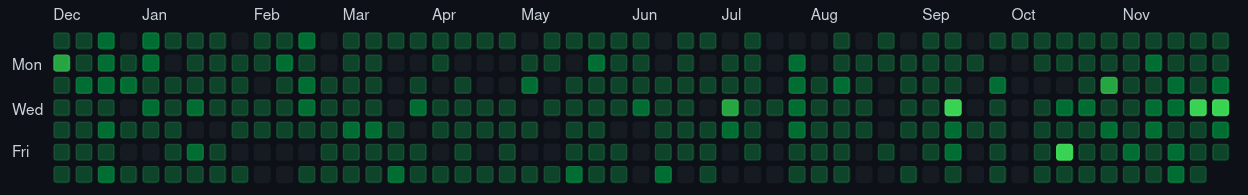
\includegraphics[width=\paperwidth]{contributions}};
\end{tikzpicture}

% personal data
\firstname{Lukas}
\familyname{Klingsbo}
\title{Freelance Software Engineer}
\homepage{https://lukas.fyi}
%\newline \small{\texttt{\textbf{Homepage: {\color{web}\weblink{http://lukas.fyi}}}}}}
%\title{BCS student of Uppsala \newline \small{\texttt{\textbf{Homepage: {\color{web}\weblink{http://www.mindlevel.net}}}}}}
%\address{Office 719 SEO\\ 851 S. Morgan St.}{Chicago, IL}
%\extrainfo{\newline \color{red}Don't miss the other pages $\rightarrow$}
\phone{+46737-42 43 45}
\email{me@lukas.fyi}
%\photo[84pt][2pt]{./profile.jpg}

%\newcommand{\up}[1]{\ensuremath{^\textrm{\scriptsize#1}}}
\nopagenumbers{}

%------------------------------------\photo[64pt][0.4pt]{picture} ----------------------------------------------
%            content
%----------------------------------------------------------------------------------
\maketitle
\section{\textbf{Experience}}
\cventry{2019 -- Now}{\textbf{Software Engineer}}{}{}{Blue Fire}
{Building open source libraries for the Flutter and Dart ecosystem, the biggest one being Flame (the Flutter game engine).}
\cventry{2017 -- 2021}{\textbf{Software Engineer}}{}{}{Klarna}
{Building the services for credit card payments and providing an uniform API to several underlaying services. Erlang and Scala.}
\cventry{2016 -- 2017}{\textbf{Software Engineer}}{}{}{DICE (EA)}
{Building scalable backend services for Battlefield 1 (the recommendations engine for example), 22M users 1.5M PSU}
\cventry{2014 -- 2015}{\textbf{Software Engineer}}{}{}{Ericsson and SICS}
{Building an information centric network in Erlang for live video streaming with an accompanying android application.
Deployed at the Skiing World Championship in Falun 2015.}
\cventry{2013}{\textbf{Lead Developer}}{}{}{London Sales (Australia)}
{Developing a large integration service for their systems. Also; an app, dashboard and CRM back-end. Mostly GWT, Java and .net.}
\cventry{2012}{\textbf{Developer}}{}{}{Kivra}
{Developing the backend for a massive online postal system, mostly in Erlang.}
\cventry{2007 -- 2013}{\textbf{Websites}}{}{}{}
{Designing and developing a lot of websites for smaller companies and stores, for example the websites of the stores \begin{math}20m^2\end{math} skor and Cri Cri.}
\cventry{2008 -- 2011}{\textbf{Developer}}{}{}{RivCalc.com}
{Developed and maintained a website written in GWT (Java syntax) to make mathematical calculations for a web-based game. Financed through google adsense.}
\cventry{2005 -- 2010}{\textbf{Tech/Computer support}}{}{}{}
{Both phone support and home visits.}
\newpage

\section{\textbf{Education}}
\cventry{2013--2015}{\textbf{Master of Computer Science}}{\newline University of Uppsala}{Sweden}{}{}
\cventry{}{\textbf{Master Thesis}}{DICE (EA)}{Uppsala}{}{
A Security Management Layer for CDN Assets}
\cventry{2009--2012}{\textbf{Bachelor of Computer Science}}{\newline University of Uppsala}{Sweden}{}{}
\cventry{}{\textbf{Bachelor Thesis}}{Kivra}{Stockholm}{}{
NoSQL: Moving from MapReduce Batch Jobs to Event-Driven Data Collection}

\section{\textbf{Open source contributions}}
\cventry{}{\textbf{Flame}}{}{}{}{
Number one contributor to Flame, the largest game engine for Flutter.}
\cventry{}{\textbf{Forge2D}}{}{}{}{
Box2D (physics engine) port for Dart.}
\cventry{}{\textbf{qmk\_firmware}}{}{}{}{
Keyboard firmware for Atmel AVR and ARM controllers.}
\cventry{}{\textbf{MindLevel}}{}{}{}{
An app with real life challanges. Kotlin (Android) front-end and Scala backend.}
\cventry{}{\textbf{Uratool}}{}{}{}{
A distributed collaborative coding editor written in Erlang.}
\cventry{}{\textbf{Esiade}}{}{}{}{
An Evolutionary simulator in a dynamic environment. Proof of concept of genetic programming and machine learning.}

\renewcommand{\cvcomputer}[2]{\cvline{#1}{\small#2}}
\section{\textbf{Preferred tools}}
\cvcomputer{OS}{Linux}
\cvcomputer{Programming}{Flutter, Dart, Scala, Erlang, Kotlin, C, Haskell, Python, Bash}
\cvcomputer{Storage}{MySql, Postgres, MongoDB, Redis, Memcached, Riak}
\cvcomputer{Editor/IDE}{Vim, IntelliJ}
\cvcomputer{Typography}{\LaTeX}
\cvcomputer{Other}{AWS Services,\newline
                   Docker,\newline
                   Git,\newline
                   Kubernetes,\newline
                   Terraform}

\newpage
\thispagestyle{empty} 
\section{\textbf{Other}}
\cventry{2006 -- Present}{\textbf{20+ Commisions of Trust}}{}{}{}{
Example: publicly elected board member of Uppsala Student Union}
\cventry{}{\textbf{Languages}}{}{}{}{English Fluently (Lived in Australia and England)\newline Swedish Mother Tounge\newline Spanish Basics (Backpacked Latin America)}
\cventry{}{\textbf{Random Facts}}{}{}{}{\begin{itemize}
  \item I have a Fork Bomb and a PRNG tattoed on my right arm.
  \item I build my own keyboards (currently use Dactyl Manuform).
  \item 2021 ranked the 28th most active GitHub user in Sweden.
\end{itemize}

\section{\textbf{Contact details}}
\cventry{E-mail}{\href{mailto:me@lukas.fyi}{me@lukas.fyi}}{}{}{}{}
\cventry{Phone}{\href{tel:+46737-42 43 45}{+46737-42 43 45}}{}{}{}{}
\cventry{Website}{\href{https://lukas.fyi}{lukas.fyi}}{}{}{}{}
\cventry{GitHub}{\href{https://github.com/spydon}{github.com/spydon}}{}{}{}{}
\cventry{Twitter}{\href{https://twitter.com/spyd0n}{twitter.com/spyd0n}}{}{}{}{}
\cventry{LinkedIn}{\href{https://www.linkedin.com/in/spydon/}{linkedin.com/in/spydon/}}{}{}{}{}

\begin{tikzpicture}[remember picture,overlay]
\node[anchor=south,opacity=0.4,inner sep=0pt] at (current page.south)
{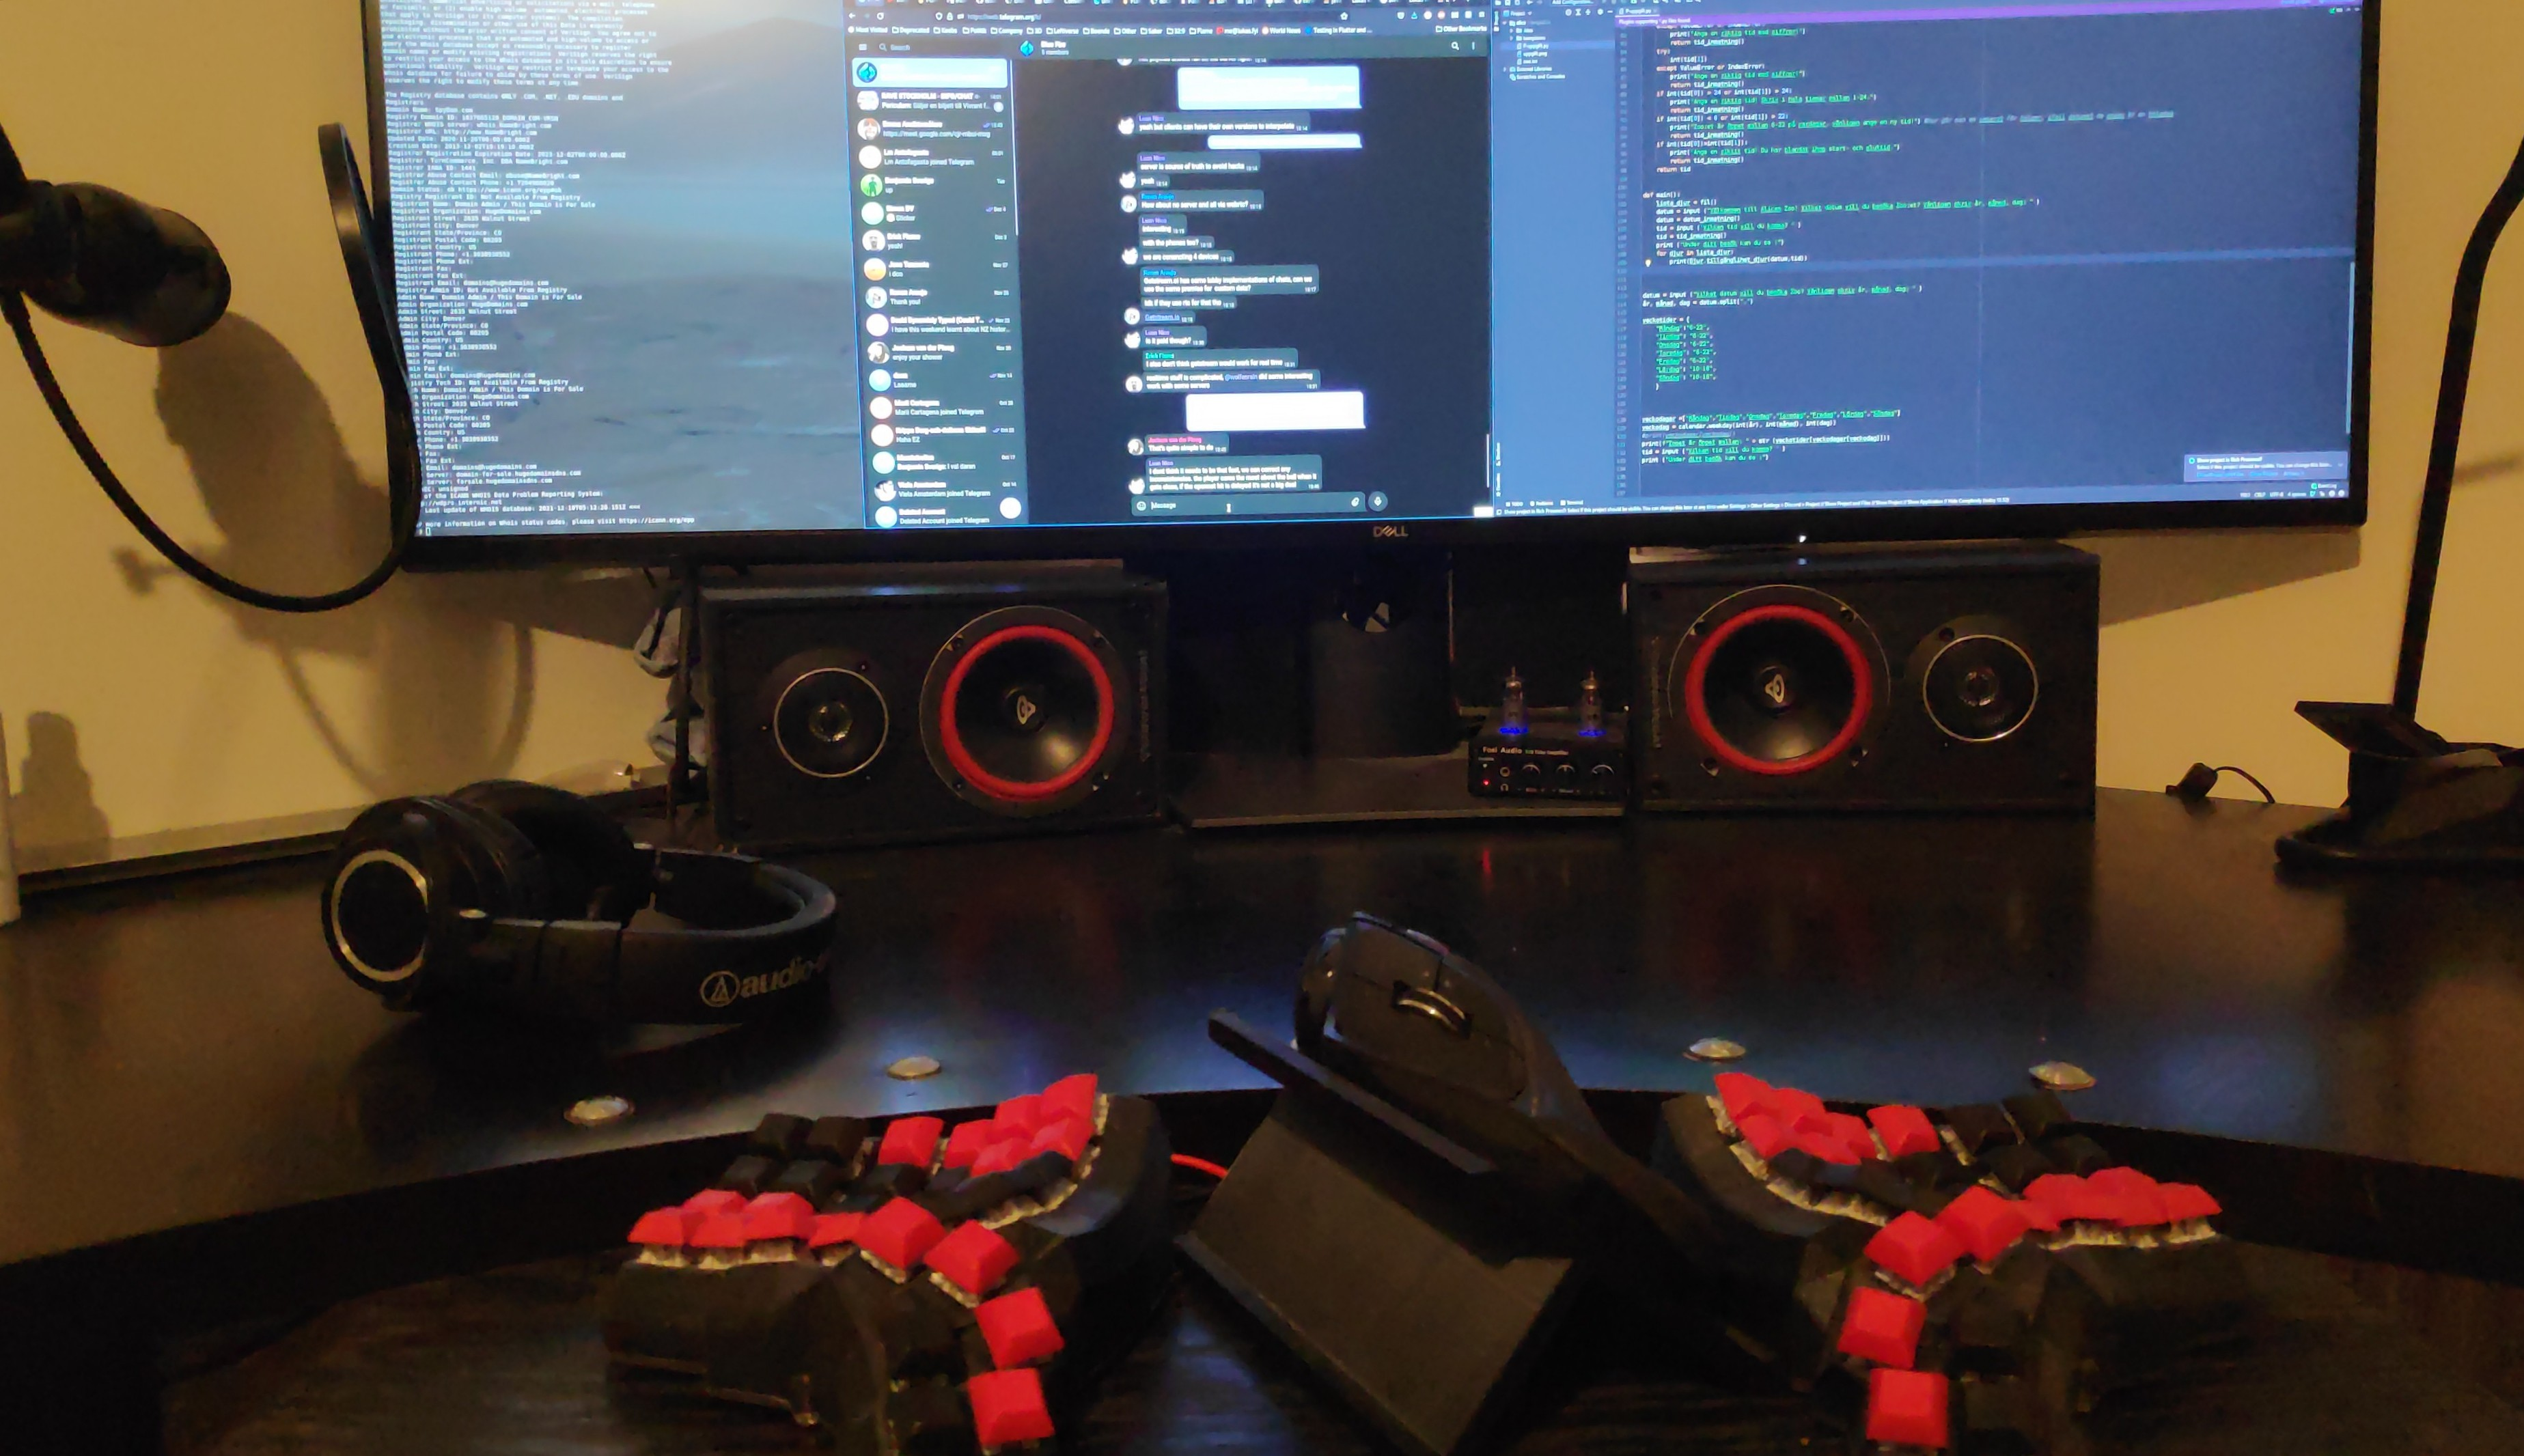
\includegraphics[width=\paperwidth]{desk}};
\end{tikzpicture}

\end{document}
